\documentclass{beamer}
\usepackage{amsmath}
\usepackage[english]{babel} %set language; note: after changing this, you need to delete all auxiliary files to recompile
\usepackage[utf8]{inputenc} %define file encoding; latin1 is the other often used option
\usepackage{csquotes} % provides context sensitive quotation facilities
\usepackage{graphicx} %allows for inserting figures
\usepackage{booktabs} % for table formatting without vertical lines
\usepackage{textcomp} % allow for example using the Euro sign with \texteuro
\usepackage{stackengine}
\usepackage{wasysym}
\usepackage{tikzsymbols}
\usepackage{textcomp}
\usepackage{xcolor}
\usepackage[dvipsnames]{xcolor}
\usepackage{colortbl}
\usepackage{adjustbox}

% ELIMINAR COMANDOS DE NAVEGACION%%%%%%%%%%%
\setbeamertemplate{navigation symbols}

%\newcommand{\bubblethis}[2]{
 %       \tikz[remember picture,baseline]{\node[anchor=base,inner sep=0,outer sep=0]%
 %       (#1) {\underline{#1}};\node[overlay,cloud callout,callout relative pointer={(0.2cm,-0.7cm)},%
 %       aspect=2.5,fill=yellow!90] at ($(#1.north)+(-0.5cm,1.6cm)$) {#2};}%
 %   }%
%\tikzset{face/.style={shape=circle,minimum size=4ex,shading=radial,outer sep=0pt,
 %       inner color=white!50!yellow,outer color= yellow!70!orange}}

%% Some commands to make the code easier
\newcommand{\emoticon}[1][]{%
  \node[face,#1] (emoticon) {};
  %% The eyes are fixed.
  \draw[fill=white] (-1ex,0ex) ..controls (-0.5ex,0.2ex)and(0.5ex,0.2ex)..
        (1ex,0.0ex) ..controls ( 1.5ex,1.5ex)and( 0.2ex,1.7ex)..
        (0ex,0.4ex) ..controls (-0.2ex,1.7ex)and(-1.5ex,1.5ex)..
        (-1ex,0ex)--cycle;}
\newcommand{\pupils}{
  %% standard pupils
  \fill[shift={(0.5ex,0.5ex)},rotate=80] 
       (0,0) ellipse (0.3ex and 0.15ex);
  \fill[shift={(-0.5ex,0.5ex)},rotate=100] 
       (0,0) ellipse (0.3ex and 0.15ex);}

\newcommand{\emoticonname}[1]{
  \node[below=1ex of emoticon,font=\footnotesize,
        minimum width=4cm]{#1};}
\usepackage{scalerel}
\usetikzlibrary{positioning}
\usepackage{xcolor,amssymb}
\newcommand\dangersignb[1][2ex]{%
  \scaleto{\stackengine{0.3pt}{\scalebox{1.1}[.9]{%
  \color{red}$\blacktriangle$}}{\tiny\bfseries !}{O}{c}{F}{F}{L}}{#1}%
}
\newcommand\dangersignw[1][2ex]{%
  \scaleto{\stackengine{0.3pt}{\scalebox{1.1}[.9]{%
  \color{red}$\blacktriangle$}}{\color{white}\tiny\bfseries !}{O}{c}{F}{F}{L}}{#1}%
}
\usepackage{fontawesome} % Social Icons
\usepackage{epstopdf} % allow embedding eps-figures
\usepackage{tikz} % allows drawing figures
\usepackage{amsmath,amssymb,amsthm} %advanced math facilities
\usepackage{lmodern} %uses font that support italic and bold at the same time
\usepackage{hyperref}
\usepackage{tikz}
\usepackage{tcolorbox}

\usefonttheme[onlymath]{serif} %set math font to serif ones

\definecolor{beamerblue}{rgb}{0.2,0.2,0.7} %define beamerblue color for later use

%%% defines highlight command to set text blue
\newcommand{\highlight}[1]{{\color{blue}{#1}}}


%%%%%%% commands defining backup slides so that frame numbering is correct

\newcommand{\backupbegin}{
   \newcounter{framenumberappendix}
   \setcounter{framenumberappendix}{\value{framenumber}}
}
\newcommand{\backupend}{
   \addtocounter{framenumberappendix}{-\value{framenumber}}
   \addtocounter{framenumber}{\value{framenumberappendix}}
}

%%%% end of defining backup slides

%Specify figure caption, see also http://tex.stackexchange.com/questions/155738/caption-package-not-working-with-beamer
\setbeamertemplate{caption}{\insertcaption} %redefines caption to remove label "Figure".
%\setbeamerfont{caption}{size=\scriptsize,shape=\itshape,series=\bfseries} %sets figure  caption bold and italic and makes it smaller

\newtcolorbox{boxA}{
    fontupper = \bf,
    boxrule = 1.5pt,
    colframe = black % frame color
}
\newtcolorbox{boxB}{
    boxrule = 1.5pt,
    colframe = blue!70!black,, % frame color
    colback = blue!7!white,
}

\usetheme{Boadilla}
% --------------------
% Overall information
% --------------------
\title[Economía I]{Economía I \vspace{4mm}
\\ Magistral 13: Fin de CP, Fin de Elasticidad y Repaso}
\date{}
\author[Franco Riottini]{Riottini Franco}
\vspace{0.4cm}
\institute[]{Universidad de San Andrés} 

\begin{document}

\begin{frame}
    \titlepage
    \centering
    
\includegraphics[scale=0.2]{../Figures/logoUDESA.jpg} 
\end{frame}

\begin{frame}
    \centering
    \begin{boxB}
    \centering \Large \textbf{Consideración Incial sobre el parcial!} \\   
    Mandamos dos mails:
    \begin{enumerate}
        \item Aula por apellido y nombre.
        \item Horario del examen.
        \item Listado de si tienen o no computadora.
    \end{enumerate}
    El que ve algo extraño con su nombre y no avisa, rinde solo la parte escrita y tiene un $0$ en todo lo demás.
    \end{boxB}
\end{frame}

\begin{frame}
    \centering
    \begin{boxB}
    \centering \Large \textbf{Competencia Perfecta en el Largo Plazo} \\   
    \end{boxB}
\end{frame}

\begin{frame}
\frametitle{¿Y en el largo plazo...?}
\begin{itemize}
\item Los beneficios extraordinarios son las ganancias de corto plazo que reciben las empresas en competencia perfecta.
    \begin{itemize}
    \item Se trata de la rentabilidad que obtienen la empresas por encima de la tasa de retorno normal (que considera todos los costos relevantes, \underline{incluyendo el costo de oportunidad del capital}).
    \end{itemize}
    \item Siempre que existan potenciales rentas (beneficios extraordinarios), va a haber firmas interesadas en entrar al mercado
    \item Si los costos de entrada no son demasiado altos, estas firmas potenciales van a entrar
    \item Al ingresar, las firmas van a presionar hacia abajo el precio de equilibrio, eliminando del mercado a las firmas menos eficientes
    \item Los beneficios que atraen a potenciales entrantes comienzan a disiparse
    \item En el largo plazo, estos beneficios van a desaparecer, serán iguales a 0.
    \end{itemize}
\end{frame}

\begin{frame}{¿Y en el largo plazo...?}
    \begin{center}
    \begin{figure} [H]
    \centering
    \tikzset{every picture/.style={line width=0.50pt}} %set default line width to 0.75pt        

    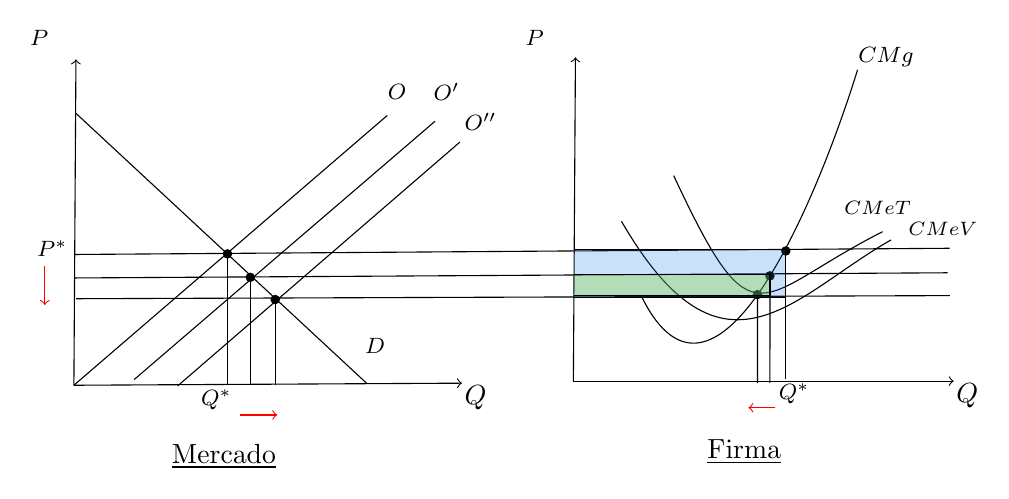
\begin{tikzpicture}[x=0.75pt,y=0.75pt,yscale=-1,xscale=1] [scale=0.8]
    %uncomment if require: \path (0,2084); %set diagram left start at 0, and has height of 2084

    %Straight Lines [id:da060960642870382165] 
    \draw    (76,1041.69) -- (216,1171.69) ;
    %Straight Lines [id:da7851707797387746] 
    \draw[->] (75,1172.69) -- (75.99,1015.69);
    %Straight Lines [id:da5252533350679736] 
    \draw[->] (75,1172.69) -- (262,1171.69);
    %Straight Lines [id:da1925274721555612] 
    \draw    (315.65,1170.69) -- (496.9,1170.69) ;
    %Straight Lines [id:da06122585785191381] 
    \draw[->]    (315.65,1170.69) -- (316.65,1014.69) ;
    \draw[->] (315.65,1170.69) -- (498.9,1170.69);
    %Straight Lines [id:da431398071619699] 
    \draw    (75,1172.69) -- (226,1042.69) ;
    %Straight Lines [id:da6076203558210751] 
    \draw [color={rgb, 255:red, 0; green, 0; blue, 0 }  ,draw opacity=1 ]   (75,1109.69) -- (496.88,1106.69) ;
    %Curve Lines [id:da8172716073565294] 
    \draw    (348.88,1130.69) .. controls (383.11,1198.69) and (430.44,1091.69) .. (452.59,1020.69) ;
    %Curve Lines [id:da7210609848314191] 
    \draw    (338.81,1093.69) .. controls (388.15,1178.69) and (422.38,1128.69) .. (468.7,1102.69) ;
    %Curve Lines [id:da02485638109474686] 
    \draw    (363.98,1071.69) .. controls (403.25,1155.69) and (403.25,1129.69) .. (464.67,1098.69) ;
    %Straight Lines [id:da9738419389002844] 
    \draw    (418,1109) -- (418,1169.69) ;
    %Straight Lines [id:da17644987359180853] 
    \draw    (149,1110) -- (149,1172.5) ;
    %Shape: Circle [id:dp2973355629068237] 
    \filldraw[black] (149,1109.39) circle (1.5pt);

    %Shape: Ellipse [id:dp8539925560604675] 
    \filldraw[black] (418,1108) circle (1.5pt); % Superior
    %Straight Lines [id:da14289261334513892] 
    \draw    (104.07,1169.91) -- (249,1045.5) ;
    %Straight Lines [id:da31165236436665356] 
    \draw    (75,1121) -- (496,1118.5) ;
    %Shape: Circle [id:dp9941417879817387]
    \filldraw[black] (160,1120.69) circle (1.5pt); 
    %Straight Lines [id:da7694650098831262] 
    \draw    (160,1118.69) -- (160,1172.5) ;
    %Straight Lines [id:da5710733904002603] 
    % \draw    (61,1112) -- (61,1127.5) ;
    \draw[->, red] (61,1115) -- (61,1134);
    %Straight Lines [id:da30346292560316446] 
    \draw    (125,1173) -- (261,1055.5) ;
    %Shape: Circle [id:dp9338937817809183]
    \filldraw[black] (172,1131.39) circle (1.5pt); 
    %Straight Lines [id:da9716189952078933] 
    \draw    (76,1131) -- (497,1129.5) ;
    %Straight Lines [id:da7462100456158596] 
    \draw    (172,1133) -- (172,1172.5) ;
    %Straight Lines [id:da6840836726821611] 
    % \draw    (155,1187) -- (171,1186.56) ;
    \draw[->, red] (155,1187) -- (173,1187);
    %Straight Lines [id:da7200406093384826] 
    \draw[->, red]    (413,1183.5) -- (400,1183.5) ;

    %Shape: Ellipse [id:dp4431909589126928] 
    % \draw  [color={rgb, 255:red, 2; green, 2; blue, 2 }  ,draw opacity=1 ][fill={rgb, 255:red, 0; green, 0; blue, 0 }  ,fill opacity=1 ] (407.09,1119.39) .. controls (407.11,1117.58) and (408.6,1116.14) .. (410.41,1116.16) .. controls (412.23,1116.18) and (413.69,1117.65) .. (413.67,1119.46) .. controls (413.65,1121.26) and (412.16,1122.71) .. (410.34,1122.69) .. controls (408.53,1122.67) and (407.07,1121.19) .. (407.09,1119.39) -- cycle ;
    \filldraw[black] (410.34,1120) circle (1.5pt); % Intermedio
    %Shape: Ellipse [id:dp8179688386007129] 
    % \draw  [color={rgb, 255:red, 2; green, 2; blue, 2 }  ,draw opacity=1 ][fill={rgb, 255:red, 0; green, 0; blue, 0 }  ,fill opacity=1 ] (401.09,1129.39) .. controls (401.11,1127.58) and (402.6,1126.14) .. (404.41,1126.16) .. controls (406.23,1126.18) and (407.69,1127.65) .. (407.67,1129.46) .. controls (407.65,1131.26) and (406.16,1132.71) .. (404.34,1132.69) .. controls (402.53,1132.67) and (401.07,1131.19) .. (401.09,1129.39) -- cycle ;
    \filldraw[black] (404.34,1129) circle (1.5pt); % Inferior
    %Shape: Rectangle [id:dp583804092155076] 
    \draw  [fill={rgb, 255:red, 18; green, 117; blue, 234 }, fill opacity=0.22 ] (316,1107.42) -- (418,1107.42) -- (418,1130.5) -- (316,1130.5) ;
    %Shape: Rectangle [id:dp5629735949679284] 
    \draw  [fill={rgb, 255:red, 126; green, 211; blue, 33 }, fill opacity=0.3 ] (316,1119.42) -- (410.38,1119.42) -- (410.38,1129.46) -- (316,1129.46) ;
    %Straight Lines [id:da14635641253383858] 
    \draw    (410.38,1129.42) -- (410.34,1171.69) ;
    %Straight Lines [id:da9761281060467815] 
    \draw    (404.38,1129.42) -- (404.34,1171.69) ;

    % Text Node
    \draw (53,1000.69) node [anchor=north west][inner sep=0.5pt]   [align=left] {\footnotesize $P$};
    % Text Node
    \draw (262,1171.69) node [anchor=north west][inner sep=0.75pt]   [align=left] {$Q$};
    % Text Node
    \draw (498.96,1170.69) node [anchor=north west][inner sep=0.75pt]   [align=left] {$Q$};
    % Text Node
    \draw (291.66,1000.69) node [anchor=north west][inner sep=0.5pt]   [align=left] {\footnotesize $P$};
    % Text Node
    \draw (225,1026.69) node [anchor=north west][inner sep=0.75pt]  [font=\footnotesize] [align=left] {\footnotesize $O$};
    % Text Node
    \draw (56,1102) node [anchor=north west][inner sep=0.75pt]  [font=\footnotesize] [align=left] {\footnotesize $P^*$};
    % Text Node
    \draw (135,1173.69) node [anchor=north west][inner sep=0.75pt]   [align=left] {\footnotesize $Q^*$};
    % Text Node
    \draw (214,1148.69) node [anchor=north west][inner sep=0.75pt]   [align=left] {\footnotesize $D$};
    % Text Node
    \draw (451.71,1008.69) node [anchor=north west][inner sep=0.75pt]   [align=left] {\footnotesize $CMg$};
    % Text Node
    \draw (444.78,1082.69) node [anchor=north west][inner sep=0.75pt]   [align=left] {\scriptsize $CMeT$};
    % Text Node
    \draw (475.79,1092.69) node [anchor=north west][inner sep=0.75pt]   [align=left] {\scriptsize $CMeV$};
    % Text Node
    \draw (413.35,1170.69) node [anchor=north west][inner sep=0.75pt]   [align=left] {\footnotesize $Q^*$};
    % Text Node
    \draw (121,1199.69) node [anchor=north west][inner sep=0.75pt]   [align=left] {\underline{Mercado}};
    % Text Node
    \draw (379,1197.69) node [anchor=north west][inner sep=0.75pt]   [align=left] {\underline{Firma}};
    % Text Node
    \draw (247,1026) node [anchor=north west][inner sep=0.75pt]  [font=\footnotesize] [align=left] {\footnotesize $O'$};
    % Text Node
    \draw (262,1040.5) node [anchor=north west][inner sep=0.75pt]  [font=\footnotesize] [align=left] {\footnotesize $O''$};
    \end{tikzpicture}
    \end{figure}
    \end{center}
\end{frame}

\begin{frame}
\frametitle{¿Y en el largo plazo...?}
\begin{figure}[h]
\tikzset{every picture/.style={line width=0.75pt}} %set default line width to 0.75pt        

\begin{tikzpicture}[x=0.75pt,y=0.75pt,yscale=-1,xscale=1] 
%uncomment if require: \path (0,1657); %set diagram left start at 0, and has height of 1657

%Straight Lines [id:da6123979361342768] 
\draw[->]     (74,298) -- (344,298) ;
%Straight Lines [id:da5131707791527922] 
\draw[->]    (74,298) -- (74,48) ;
%Straight Lines [id:da6346804843028921] 
\draw    (75,188) -- (334,189) ;
%Curve Lines [id:da697350144213293] 
\draw    (109,126) .. controls (142,212) and (270,204) .. (297,123) ;
%Curve Lines [id:da9799910224345574] 
\draw    (112,229) .. controls (136,295) and (246,141) .. (271,95) ;
%Straight Lines [id:da5845279516726063] 
\draw    (204.5,188.5) -- (204,297) ;

% Text Node
\draw (45,35) node [anchor=north west][inner sep=0.5pt]   [align=left] {$P$};
% Text Node
\draw (346,298) node [anchor=north west][inner sep=0.75pt]   [align=left] {$q$};
% Text Node
\draw (297,123) node [anchor=north west][inner sep=0.75pt]   [align=left] {$CMeT$};
% Text Node
\draw (271,85) node [anchor=north west][inner sep=0.75pt]   [align=left] {$CMg$};
% Text Node
\draw (50,178) node [anchor=north west][inner sep=0.75pt]   [align=left] {$P^*$};
% Text Node
\draw (194,299) node [anchor=north west][inner sep=0.75pt]   [align=left] {$q^*$};
\end{tikzpicture}
\end{figure}
\end{frame}

\begin{frame}
\frametitle{¿Y en el largo plazo...?}
\begin{itemize}
    \item Vimos que en el equilibrio a largo plazo, el precio $P$ es igual al costo marginal $CMg$, por lo que la empresa maximiza sus beneficios. El precio también es igual al costo total promedio $CTMe$, por lo que los beneficios son cero.
    \item ¿Qué implica esto? Que las empresas en el largo plazo operan en su escala eficiente!
    \item Recuerden que el $CMg$ se iguala con el $CTMe$  solo cuando la empresa opera en el mínimo de su costo total promedio.
\end{itemize}
\end{frame}

\begin{frame}
\frametitle{¿Por qué es eficiente?}
\begin{itemize}
    \item Los participantes son tomadores de precios
    \begin{itemize}
        \item No hay poder de mercado.
        \item La competencia impide a los vendedores aumentar el precio, y a los compradores bajarlo.
    \end{itemize}
    \item No hay barreras de entrada
    \item Los contratos son completos
        \begin{itemize}
        \item Los detalles del intercambio pueden ser definidos en forma clara, y estos contratos se pueden hacer cumplir.
        \end{itemize}
    \item No hay externalidades
        \begin{itemize}
        \item La transacción sólo afecta a los compradores y vendedores
        \end{itemize}
\end{itemize}
\end{frame}

\begin{frame}
\frametitle{Conclusión de largo plazo}

\begin{itemize}
\item ¿Por qué las empresas competitivas siguen operando si obtienen cero beneficios?
\item Recuerden la distinción entre beneficios contables y beneficios económicos. Estos últimos incluyen todos los costos de oportunidad de la empresa.
\item En el equilibrio de cero beneficios, los ingresos de la empresa deben compensar a los propietarios por estos costos de oportunidad.

\end{itemize}
\end{frame}

\begin{frame}
    \centering
    \begin{boxB}
    \centering \Large \textbf{Volvemos a Elasticidad Rápido} \\   
    \end{boxB}
\end{frame}

\begin{frame}{Elasticidad Cruzada}
    \begin{itemize}
        \item Es el cambio porcentual en las cantidades demandadas cuando \textbf{el precio de otro bien} cambia 1\%.
        \begin{equation*}
            \epsilon_{x,y} = \frac{\Delta \% Q_x}{\Delta \% P_y}
        \end{equation*}
            \begin{itemize}
            \item Si la elasticidad cruzada es 0, no hay relación entre ambos bienes.
            \item Si esta elasticidad es mayor a 0, los bienes son sustitutos, es decir, cuando se incrementa el precio de y aumenta la cantidad demandada de x; 
            \item Si es menor a 0, los bienes son complementarios, es decir, si aumenta el precio de y baja la cantidad demandada de x.
            \end{itemize}
        \item En este caso, es necesario no usar módulo porque es justamente el signo lo que nos ayuda a interpretar qué tipo de bienes son.
    \end{itemize}
\end{frame}

\begin{frame}{Elasticidad Ingreso}
  \begin{itemize}
    \item Es el cambio porcentual en las cantidades demandadas cuando el \textbf{ingreso} cambia 1\%.
    \begin{equation*}
      \epsilon_I = \frac{\Delta \% Q}{\Delta \% I}
    \end{equation*}    
    \begin{itemize}
        \item Si la elasticidad ingreso es mayor a 0, significa que ingreso y cantidades se mueven en conjunto, por lo que se trata de bienes normales.
        \item Si la elasticidad ingreso es menor a cero, ante un cambio en el ingreso la cantidad demandada del bien se mueve en la dirección opuesta. En este caso estamos en presencia de un bien inferior.
        \item Si la elasticidad ingreso es mayor a 1 decimos que estamos ante un bien de lujo.
    \end{itemize}
    \item  En este caso, al igual que con la elasticidad cruzada, es necesario no usar módulo porque es justamente el signo lo que nos ayuda a interpretar qué tipo de bienes son.
\end{itemize}
\end{frame}

\begin{frame}
    \centering
    \begin{boxB}
    \centering \Large \textbf{Repasamos Teoría de Juegos} \\   
    \end{boxB}
\end{frame}

\begin{frame}
\frametitle{Repaso: Teoría de Juegos}
    ¿Cuál es la \textbf{mejor respuesta} de cada individuo?
    \begin{itemize}
        \item  Se denomina mejor respuesta a aquella estrategia que proporciona al jugador el pago más elevado, condicional a lo que se conjetura que harán los demás
    \end{itemize}
    \vspace{2mm}
    ¿Qué es una \textbf{estrategia dominante}?
    \begin{itemize}
        \item  Una estrategia dominante es una mejor respuesta a todas las posibles estrategias de otro jugador. Si un agente tiene una estrategia dominante \textbf{siempre} la va a jugar, independientemente de la estrategia que juegue el rival.
        \item Si se encuentra un resultado donde cada individuo juega su estrategia dominante, entonces nos encontramos con un equilibrio en estrategia dominante.
        \end{itemize}
\end{frame}

\begin{frame}
\frametitle{Repaso: Teoría de Juegos}
\textbf{Equilibrio de Nash}
    \begin{itemize}
        \item  Un perfil de estrategias es un equilibrio de Nash si, dadas las estrategias del rival, cada uno de los agentes está jugando su mejor respuesta.
    \end{itemize}
    \begin{boxB}
        \centering
        En un equilibrio de Nash, ninguno de los jugadores tiene incentivos a desviarse, debido a que no puede obtener un pago mayor cambiando de estrategia.
    \end{boxB}
   \textbf{ Equilibrio Pareto eficiente}
        \begin{itemize}
        \item   En un equilibrio Pareto eficiente, no hay otra situación o alternativa en donde uno esté mejor y ninguno esté peor. 
    \end{itemize}

\end{frame}

\begin{frame}{Ejercicio - Teoría de Juegos}
Dos empresas rivales, A y B, venden productos similares. Ambas están evaluando si gastar en una costosa campaña publicitaria o no. La publicidad aumenta significativamente sus ventas si la otra empresa no hace publicidad. Pero si ambas hacen publicidad, el gasto se neutraliza y las ganancias son menores. Si ninguna hace publicidad, ambas mantienen sus clientes actuales.
    \begin{itemize}
        \item El costo de hacer publicidad es de \$3.000 para la empresa A y \$2.000 para la empresa B.
        \item Si \textbf{solo una empresa} hace publicidad, esa empresa gana \$10.000 en ventas, mientras que la otra solo gana \$2.000.
        \item Si \textbf{ambas hacen publicidad}, cada una gana \$6.000 en ventas.
        \item Si \textbf{ninguna hace publicidad}, cada una gana \$5.000.
    \end{itemize}
\end{frame}

\begin{frame}
\frametitle{Ejercicio - Teoría de Juegos}
\begin{enumerate}
    \item Construir la matriz de pagos con las ganancias netas.
    \item Identificar, si lo hay, el Equilibrio de Nash.
    \item ¿Hay estrategias dominantes para alguna de las empresas?
    \item Si hay equilibrio de Nash ¿es Pareto eficiente?
\end{enumerate}
\end{frame}

\begin{frame}
\frametitle{Ejercicio - Teoría de Juegos}
\begin{center}
\renewcommand{\arraystretch}{1.8} % <-- Espaciado vertical
\begin{tabular}{c|c|c}
 & \textbf{B: Publicidad} & \textbf{B: No Publicidad} \\
\hline
\textbf{A: Publicidad} & (3.000,\ 4.000) & (7.000,\ 2.000) \\
\textbf{A: No Publicidad} & (2.000,\ 8.000) & (5.000,\ 5.000) \\
\end{tabular}
\end{center}
\end{frame}

\begin{frame}
    \centering
    \begin{boxB}
    \centering \Large \textbf{Ping Pong de Verdaderos/Falsos} \\   
    \end{boxB}
\end{frame}

\begin{frame}
\frametitle{Ping Pong de Verdaderos/Falsos}
\centering
Si el objetivo de la empresa fuera maximizar los ingresos totales, la empresa debería disminuir el precio si se encuentra en un punto de la curva de demanda con elasticidad precio mayor a 1
\end{frame}

\begin{frame}
\frametitle{Ping Pong de Verdaderos/Falsos}
\centering
A una empresa en un mercado de competencia perfecta nunca le conviene seguir produciendo si su precio es menor al costo medio total porque tendría pérdidas
\end{frame}

\begin{frame}{Ping Pong de Verdaderos/Falsos}
    \centering
    El efecto sustitución siempre actúa en dirección opuesta al cambio de precio, mientras que el efecto ingreso puede reforzarlo o contrarrestarlo.
\end{frame}

\begin{frame}{Ping Pong de Verdaderos/Falsos}
    \centering
    En todo el mundo se comen hamburguesas. Sin embargo, las campañas que promueven el vegetarianismo están afectando su popularidad entre los consumidores. A la vez, el precio de la carne aumentó debido a restricciones productivas. Esto genera que tanto el precio como la cantidad de equilibrio de hamburguesas caigan. 
\end{frame}

\begin{frame}{Ping Pong de Verdaderos/Falsos}
    \centering
    Dado un determinado nivel de cantidades, si la valoración social es más alta que el costo marginal que tienen las empresas en ese punto, entonces el precio de equilibrio es mayor al que se esté observando.
\end{frame}

\begin{frame}{Ping Pong de Verdaderos/Falsos}
    \centering
    La empresa Whirlpool produce heladeras y se enfrenta a una competencia fuerte. La empresa tiene una elasticidad cruzada con respecto al precio al que vende la empresa Electrolux de 0.5 y una elasticidad cruzada del precio al que vende la empresa LG de 1.2. Esto implica que Whirlpool prefiere que Electrolux baje sus precios.
\end{frame}

\begin{frame}{Descomposición del Efecto Precio en Efecto Sustitución y Efecto Ingreso}
    \scriptsize
    Suponga que Julia consume únicamente dos bienes: Pizza (bien X) y Entradas al Cine (bien Y). Julia tiene un ingreso semanal de \$600. El precio inicial de una pizza es \$30 y el precio inicial de una entrada al cine es \$20. Actualmente, Julia elige consumir 10 pizzas y 15 entradas al cine cada semana.
    Debido a una reducción en el precio de la pizza, ahora cada pizza cuesta solo \$20, manteniéndose constante tanto el precio del cine (\$20) como el ingreso semanal de Julia (\$600). Tras esta reducción en el precio, Julia modifica su consumo y ahora compra 15 pizzas y 15 entradas al cine.
    \begin{enumerate}
        \item Dibuje cuidadosamente el gráfico presupuestario original y el nuevo tras la reducción en el precio de la pizza. Indique claramente los interceptos y la pendiente en ambos casos. Indique el punto inicial y final del consumo de Julia.
        \item Indique gráficamente cómo se descompone el cambio total en dos componentes: efecto sustitución y efecto ingreso. Responda:
        \begin{itemize}
            \scriptsize
            \item ¿Qué significa el efecto sustitución para el consumo de pizza? ¿Como se relaciona con el efecto sustitución en el consumo de entradas al cine?
            \item ¿Qué significa el efecto ingreso para el consumo de pizza? ¿Como se relaciona con el efecto ingreso en el consumo de entradas al cine?
        \end{itemize}
    \end{enumerate}
\end{frame}

\end{document}